%
% A brief introduction of evolutionary algorithm, Zhang Jiadong, 2017
%

\documentclass[10pt]{beamer}

\usetheme{metropolis}
\usepackage{appendixnumberbeamer}

\usepackage{booktabs}
\usepackage[scale=2]{ccicons}
\usepackage{listings}
\usepackage{tikz}
\usepackage[BoldFont,SlantFont,CJKchecksingle]{xeCJK}
\setCJKmainfont[BoldFont=SimHei,SlantedFont=KaiTi]{SimSun}
\setCJKsansfont[BoldFont=SimHei,SlantedFont=KaiTi]{SimSun}
\setCJKmonofont[ItalicFont={Adobe Fangsong Std}]{SimSun}
\setCJKfamilyfont{zhsong}{SimSun}
\setCJKfamilyfont{zhhei}{SimHei}
\setCJKfamilyfont{zhkai}{KaiTi}
\setCJKfamilyfont{zhfs}{FangSong}

\usepackage{pgfplots}
\usepgfplotslibrary{dateplot}

\usepackage[linesnumbered,ruled]{algorithm2e}
\usepackage{algorithmicx}
\usepackage{algpseudocode}
\usepackage{amsmath}
\usepackage{graphicx}

\usepackage{xspace}
\newcommand{\themename}{\textbf{\textsc{metropolis}}\xspace}

\title{进化算法简介}
%\subtitle{A modern beamer theme}
\date{\today}
\author{马春雨 \ 马芮 \ 葛丛丛 \\ 刘汶鑫 \ 张毅 \ 张甲栋}
\institute{浙江大学计算机科学与技术学院}
%\titlegraphic{\hfill\includegraphics[height=1.5cm]{logo.pdf}}

\begin{document}

\maketitle

\begin{frame}{目录}
  \setbeamertemplate{section in toc}[sections numbered]
  \tableofcontents[hideallsubsections]
\end{frame}

%\section{前言}
%
%\begin{frame}[fragile]{前言}
%
%	进化算法是以达尔文的进化论思想为基础,通过模拟生物进化过程与机制的求解问题的自组织、自适应的人工智能技术。
%	
%\end{frame}

%topics

%
% GNU courseware, Zhang Jiadong, 2018
%

\section{前言}\fontsize{12pt}{12pt}\selectfont

\frame{\frametitle{定义}
又叫演化计算,是模拟自然界中的生物的演化过程产生的一种群体导向的随机搜索技术和方法。

~

是一种通用的问题求解方法,具有自组织、自适应、自学习性和本质并行性等特点,
不受搜索空间限制性条件的约束,也不需要其它辅助信息。
}

\frame{\frametitle{思想}
进化算法是受生物进化过程中“优胜劣汰”的自然选择机制和遗传信息的传递规律的影响,
通过程序迭代模拟这一过程,把要解决的问题看作环境,在一些可能的解组成的种群中,
通过自然演化寻求最优解。
}

\frame{\frametitle{种类}
	\begin{itemize}
		\item<1-> 遗传算法(Genetic Algorithms)
		\item<2-> 演化策略(Evolution Strategy)
		\item<3-> 演化规划(Evolution Programming)
		\item<4-> 遗传程序设计(Genetic Programming)
		\item<5-> 多种群协同进化(Coevolutionary Algorithm)
		\item<6-> 差分进化算法(Differential Evolutionary)
	\end{itemize}
}

%end

%
% GNU courseware, XIN YUAN, 2017
%

\section{遗传算法}

\frame{\frametitle{遗传算法}
	\begin{itemize}
		\item<1-> 遗传算法概述
		\item<2-> 遗传算法原理
		\item<3-> 遗传算法应用
	\end{itemize}
}

\frame{\frametitle{遗传算法概述}
\ \ \ \ 遗传算法模拟自然选择和自然遗传过程中发生的繁\\
殖、交叉和基因突变现象,在每次迭代中都保留一组候\\
选解,并按某种指标从解群中选取较优的个体,利用遗\\
传算子(选择、交叉和变异)对这些个体进行组合,产生\\
新一代的候选解群,重复此过程,直到满足某种收敛指\\标为止。
}


\frame{\frametitle{基本遗传算法}
\ \ \ \ \ \ 基本遗传算法(Simple Genetic Algorithms,\\
简称SGA,又称简单遗传算法或标准遗传算法),\\
是由Goldberg总结出的一种最基本的遗传算法,\\
其遗传进化操作过程简单,容易理解,是其它一\\
些遗传算法的雏形和基础。 
}


\frame{\frametitle{遗传算法过程}
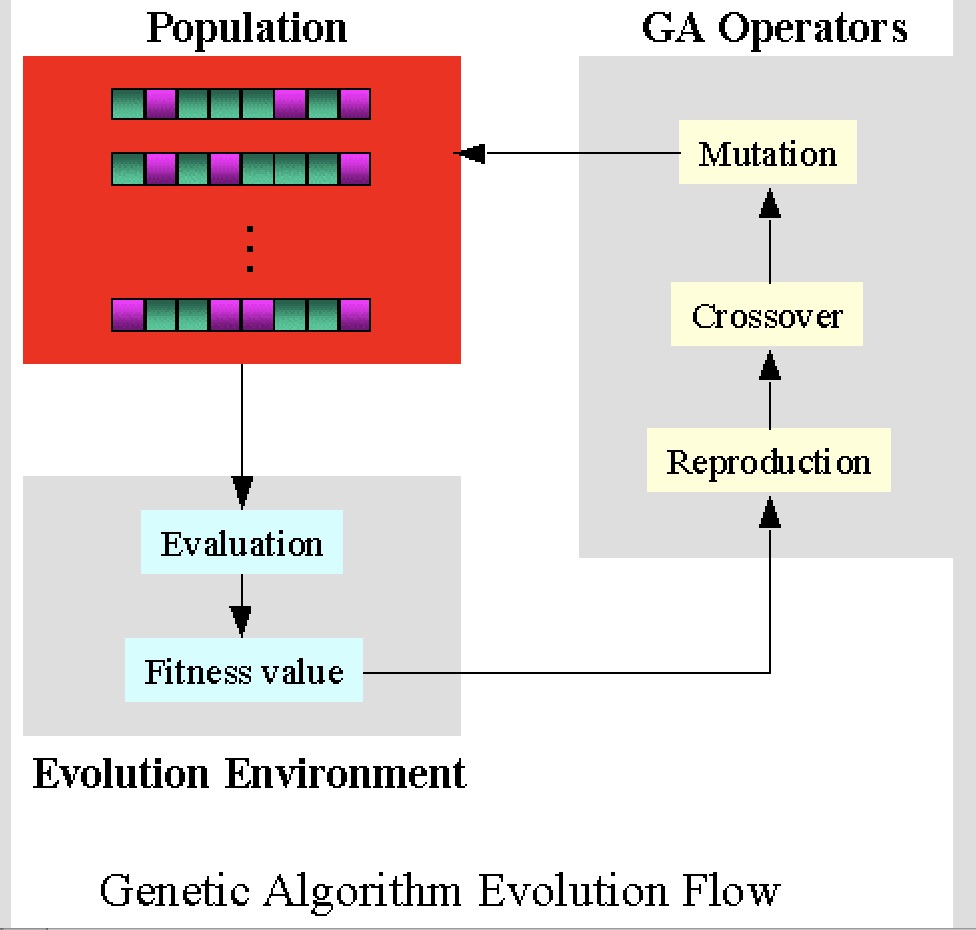
\includegraphics[width=0.8\textwidth]{evolutionflow.jpg}
}

\frame{\frametitle{基本遗传算法的组成}
(1)编码:通过某种编码机制把对象抽象
为由特定符号按一定顺序排成的串。
SGA使用二进制串进行编码。 \\
(2)适应度函数:遗传算法对一个个体(解)
的好坏用适应度函数值来评价,适应度函数值越大,解的质量越好。\\

}

\frame{\frametitle{基本遗传算法的组成}
(3)遗传算子(选择、交叉、变异)\\
选择算子:优胜劣汰操作,适应度高的个体被遗传到下一代群体中的概率大;
适应度低的个体,被遗传到下一代群体中的概率小。SGA中选择算子采用轮盘
赌选择方法。\\
交叉:对两个相互配对的染色体依据交叉概率 Pc 按某种方式相互交换其部分
基因,从而形成两个新的个体。SGA中交叉算子采用单点交叉算子。\\
变异算子: 依据变异概率 Pm 将个体编码串中的某些基因值用其它基因
值来替换,从而形成一个新的个体 。SGA中变异算子采用基本位变异算子。\\
}

\frame{\frametitle{基本遗传算法的组成}
(4)运行参数\\
M  : 种群规模 \\
T  : 遗传运算的终止进化代数 \\
Pc  : 交叉概率 \\
Pm : 变异概率 \\
}

\frame{\frametitle{遗传算法原理}
模式定理:具有低阶、短定义距以及平均适应度高于种群平均适应度的模式在子代中呈指数增长。\\

积木块假设:遗传算法通过短定义距、低阶以及高平均适应度的模式(积木块),在遗传操作下相互
结合,最终接近全局最优解。\\

模式定理保证了较优模式的样本数呈指数增长,从而使遗传算法找到全局最优解的可能性存在;\\
而积木块假设则指出了在遗传算子的作用下,能生成全局最优解。 \\

}

\frame{\frametitle{遗传算法应用}
(1)组合优化     (2)函数优化\\ 
(3)自动控制     (4)生产调度\\
(5)图像处理      (6)机器学习\\
(7)人工生命      (8)数据挖掘\\
}

%end

%
% GNU courseware, XIN YUAN, 2017
%

\section{演化策略}

\frame{
\centerline{\textbf{\Huge{演化策略}}}
}

\frame{\frametitle{定义}

\begin{block}{定义}
%它与遗传算法类似,但是它用实值参数代替二进制串
演化策略(Evolutionary Strategy ,ES) 是最古老的演化算法之一,而且非常有效。演化策略是20世纪60年代由柏林工业大学的Rechenberg和Schwefel提出来的(和遗传算法同时代提出),演化策略的设计之初是想用来解决流体力学问题,目前已形成演化计算的一个重要分支。演化策略主要用于连续参数优化问题。
\end{block}
}
\frame{\frametitle{演化策略与遗传算法的区别}
%演化策略(Evolution Strategies)和遗传算法(Genetic Algorithms)最基本的不同在于它们各自的应用领域。演化策略的开发是针对数值优化,它采用一特殊的带自适应步长大小和倾角的爬山过程。最近,演化策略已经用语离散的优化问题。而遗传算法是作为(一般目的)自适应搜索技术形成的,这种搜索技术按指数增长的比率分配平均值之上的模式。它能用在各种领域,(实)参数优化只是它应用中的个方面。
\begin{block}{一、表达个体的方式}
演化策略:操作于浮点向量。      
\\经典遗传算法:操作于二进制向量。
\end{block}

\begin{block}{二、选择过程本身}
在演化策略里,选择过程是确定性的,选择没有重复。
\\在遗传算法里,选择过程是随机的,选择有重复,选择的机会与个体的适应值成比例。一些遗传算法实际上使用了分级加权选择,但较强个体仍可以被选择几次。
\end{block}

\begin{block}{三、选择和重组步骤的相对次序}
在演化策略里,一个后代是两个亲体杂交和进一步交异的结果,u+y 或 y 个个体组成的中间群体已准备好,选择过程减少其大小到 u 个个体。
\\在遗传算法中,次序正好相反。我们首先选择一些中间群体,然后应用遗传算子(杂交和变异)到一些个体上(按照杂交概率选择)及一些基因上(按照变异概率选择)。
\end{block}
}

\frame{\frametitle{演化策略与遗传算法的区别}
\begin{block}{四、控制参数}
遗传算法在演化过程中再生殖参数保持常数(杂交概率、变异概率)
\\演化策略始终改变参数(自适应步长 和倾角):它们和解向量x一起经历杂交和变异,因为一个个体被解释为这三个参数的三位一体(x,自适应步长,倾角)。演化策略中控制参数的自适应对应于系统的局部微调。
\end{block}

\begin{block}{五、处理约束}
演化策略承担一组q≥0个不等式,G1(x)>=0,...,Gq(x)>=0作为优化问题的一部分。在一些迭代过程中,如果一个后代不满足所有这些约束,那么此后代消亡,即不被放到新群体中。如果这样的非法个体发生率很高,演化策略就调整它们的控制参数,即减少向量 的部分。
\\遗传算法处理约束的主要策略是对违反约束的个体加以惩罚。理由是对强约束问题,不能只是消去不合法后代(遗传算法不调节它们的控制参数),否则,算法将长时间原地不动。走进细看演化策略的遗传算法在过去20年的发展,人们不得不承认,这些方法之间的鸿沟正变得越来越小。
\end{block}

}
\frame{\frametitle{演化策略的一般结构}
早期的演化策略种群中只包含一个个体,称之为父体。在演化过程中,仅有一种遗传算子变异。在每代一演化后,通过将变异算子应用到父体上得到一个后代,然后将后代与父体进行比较,若后代比父体好且满足所有的约束条件,则后代成为下一代种群中的父体,否则父体保持不变。这种演化策略称为(1+1)演化策略。
}

\frame{\frametitle{演化策略的一般结构}
(1+1)演化策略没有体现种群的作用,本质上是一种局部搜索策略,具有明显的局限性。

\begin{itemize}
		\item<1-> 随后,Rechenberg又提出了($\mu$+1)-演化策略。
		
		\item<2-> 后来Schwefel又提出了($\mu$+$\lambda$)演化策略和($\mu$,$\lambda$)演化策略。
		
	\end{itemize}

}

\frame{\frametitle{应用实例}
\begin{itemize}
		\item<1-> 考虑下面的Ackley函数极小化问题
		\\
		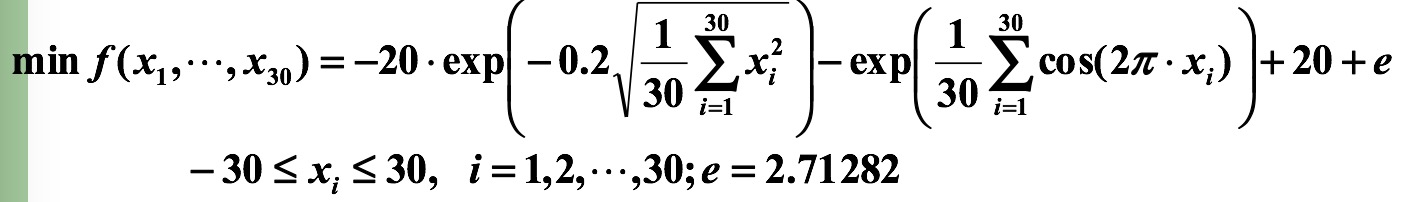
\includegraphics[width=0.8\textwidth]{algorithm.jpg}
		
		\item<2-> 求解该问题的演化策略设计如下:
		  \begin{itemize}
		     \item<1-> 表示
		\\
		       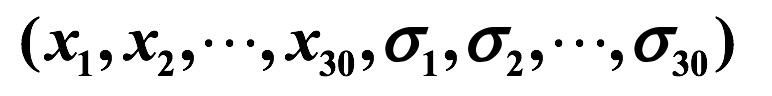
\includegraphics[width=0.8\textwidth]{algorithm2.jpg}
		     \item<2-> 适应函数:适应函数取为目标函数。
		     \item<3-> 重组算子:对变量部分使用离散重组,对策略参数部分使用全局中值重组。 
		     \item<4-> 存活选择:使用($\mu$,$\lambda$)选择,其中$\mu$=30,$\lambda$)=200。
		     \item<5-> 终止准则:当进行200000次函数值计算或发现最优解后终止算法。
		     \item<6-> 种群初始化:初始种群中每个个体的变量部分随机地产生,每个分量均匀地分布在区间       内。每个个体的变异步长都相同,设为$\theta$=3。  
	
	      \end{itemize}
		\item<3-> 运行上述算法10次,每次找到的最好解都位于全局最优峰上。

		
	\end{itemize}


   

}





%end

%
% GNU courseware, XIN YUAN, 2017
%

\section{演化规划}\fontsize{12pt}{12pt}\selectfont

%\frame{
%\centerline{\textbf{\Huge{演化规划}}}
%}

\frame{\frametitle{定义}

\begin{block}{定义}
%From Wikipedia:\\Evolutionary programming is one of the four major evolutionary algorithm paradigms. It is similar to genetic programming, but the structure of the program to be optimized is fixed, while its numerical parameters are allowed to evolve.进化规划是四种主要的演化算法之一。 它与遗传算法类似,但要优化的程序结构是固定的,而其数值参数则可以进化。
~

演化规划(Evolutionary Programming Algorithm, EPA)是由美国学者Lawrence J. Fogel于1960年提出的,它适用于解决目标函数或约束条件不可微的复杂非线性实值连续优化问题。它与遗传算法类似,但要优化的程序结构是固定的,而其数值参数则可以进化。
\end{block}
}
\begin{algorithm}
\caption{Evolutionary Programming Algorithm}
    \KwIn{个体表现型$X$, 群体规模$N$, 迭代次数$G$等}
    \KwOut{子代}
    	随机产生初始群体并计算适应值(含$N$个个体)\\
        \While{not done}{
        //终止条件:达到规定的进化代数,或若干代内种群中最好个体的函数值不再发生变化,则终止进化\\
        	\For{$\rm i = 1;i < N; i++$}
        	{
           		对$X_i$进行变异得到$X_i'$\\
				对$X_i$进行可行性检查\\
				计算$X_i$的适应值\\

        	}
        	从$2N$个个体中选择$N$个个体 //随机型q-竞争法\\
        }
        return 子代\;
\end{algorithm}
\frame{\frametitle{思想}
EP模拟生物种群层次上的进化,因此在进化过程中主要强调生物种群行为上的联系,即强调种群层次上的行为进化而建立父、子代间的行为链。
~

EP算法最重要的一个操作是变异操作。通过变异,父代群体中的每一个个体产生一个子代个体,父代和子代中最好的那一半被选择生存下来。
}

\frame{\frametitle{q-竞争选择算法}
演化规划算法的选择策略采用的是q-竞争机制,这也是与进化策略算法最大的不同点,q-竞争说白了就是选择优质解的同时,以一定的随机概率接受较差的解。多数是优解,少数是比较差的解,共同组成一组父代,为下一次进化做准备。
}

\frame{\frametitle{q-竞争选择算法}
\textbf{思想}\\
将N个父代进化的N个子代一起放在一起,从中随机选择不重复q个个体组成一个组,然后依次对2N个个体的每一个个体进行计分,将2N个依次每次一个与随机挑选出的群组的每一个成员进行比较,相比优的话,则会对应的个体的分数加1,最后对分数进行排序,选择分数最高的N个个体!
}

\frame{\frametitle{缺点}
	大量的研究证明,由于过度选择、变异操作破坏有效模式、参数选取不当等原因,该算法存在一些亟待克服
的\textbf{缺点}:\\
(1)容易出现早熟收敛现象\\
(2)进化后期,个体之间的竞争趋缓导致算法后期的搜索效率降低等。
}

\frame{\frametitle{改进}
	\begin{itemize}
		\item<1-> 基于柯西变异的进化规划算法 1996
		% 该算法能够较好地克服早熟收敛现象,但是后期搜索的效率很低
		\item<2-> 基于Lévy概率分布的进化规划算法(LEP) 2004
		% 在该算法中使用Lévy分布变异算子代替高斯分布变异算子,其思想是使用具有更大方差的变异算子来促使种群更快地收敛到最优解,但编制Lévy 算子较为困难,且使用大方差的变异算子使种群收敛到最优解的速度变慢。
		\item<3-> 一种求解数值优化问题的快速进化规划算法 2004
		% 在该算法中,对变异算子进行了改进,对成功的变异进行适当延伸,当个体变异失败时,对变异量实施Gauss或Cauchy扰动,其思想是利用高斯变异算子良好的局部搜索能力和柯西变异算子良好的全局探索能力,以期能快速收敛到最优解。但是同时使用两种变异方式,导致算法的计算复杂度增加,算法的收敛速度受到影响
		\item<4-> ... 
	\end{itemize}
}

%end

%
% GNU courseware, XIN YUAN, 2017
%

\section{遗传程序设计}

%\frame{
%\centerline{\textbf{\Huge{遗传程序设计}}}
%}

\frame{\frametitle{背景}
\parindent=19pt	
\renewcommand{\raggedright}{\leftskip=0pt \rightskip=0pt plus 0cm}
\raggedright
自计算机出现以来,计算机科学的一个方向性目标就是让计算机自主进行程序设计,即只要告诉计算机要解决的问题,而不需要告诉它具体如何去做。遗传程序设计便是在该领域的一种尝试。

遗传程序设计最早由John Holland的遗传算法衍生而来,是一种由生物学引发的不依赖于领域的方法,它从问题需求的高层次描述中自动地产生计算机程序。

20世纪80年代以来,演化计算成为国际上诸多领域研究的热点。作为演化计算最新的分支,遗传程序设计(GP)自1990年前后提出后便成为广大学者关注的方向。
}

\frame{\frametitle{研究现状}
\parindent=19pt	
\renewcommand{\raggedright}{\leftskip=0pt \rightskip=0pt plus 0cm}
\raggedright	
目前在国外,GP在某些方面已经进入了应用性研究的阶段。在模拟与数字电路设计与分布式模糊控制方面,用GP自动设计的成果已经有了相当优良的性能。

国内对GP的研究起源于1990年前后,现在已开始成为诸多领域的研究热点。武汉大学软件工程国际重点实验室在动态系统的演化建模方面具有国际领先的水平。
}

\frame{\frametitle{定义}
\parindent=19pt	
\renewcommand{\raggedright}{\leftskip=0pt \rightskip=0pt plus 0cm}
\raggedright
遗传程序设计简称GP,是一种从生物演化过程得到灵感的自动化生成和选择计算机程序来完成用户定义的任务的技术。
}

\frame{\frametitle{原理}
\parindent=19pt	
\renewcommand{\raggedright}{\leftskip=0pt \rightskip=0pt plus 0cm}
\raggedright	
遗传程序设计借助达尔文进化论中适者生存的理论,模拟自然界生物体的自然选择和进化的过程,从产生一个随机的计算机程序群体出发,以适应值度量为衡量计算机程序解决特定问题好坏的标准,基于适应值按概率方式从群体中选出计算机程序进行复制和杂交等操作,以适当的停止准则终止循环,迭代执行其中的每一个计算机程序,在可能的计算机程序空间中寻找适应性最好的程序,最终获得对特定输入产生所要求输出的计算机程序。
}

\frame{\frametitle{对象}
\parindent=19pt	
\renewcommand{\raggedright}{\leftskip=0pt \rightskip=0pt plus 0cm}
\raggedright
与传统的数值优化算法不同,遗传程序设计的操作对象是规模和形状都能够动态变化的具有分层结构的计算机程序,从而不再局限于数值优化的范畴。
}

\frame{\frametitle{优点}
\parindent=19pt	
\renewcommand{\raggedright}{\leftskip=0pt \rightskip=0pt plus 0cm}
\raggedright	
遗传程序设计由已知的数据在适应值度量的推动下推导出其内在的未知规律即程序,避免了对求解过程的限制和先验性假设的要求。
}

\frame{\frametitle{框架}
\parindent=19pt	
\renewcommand{\raggedright}{\leftskip=0pt \rightskip=0pt plus 0cm}
\raggedright	
对程序设计问题,先产生一个不费事的有错误的解,然后再修改使它正确工作,这种做法一般要比坚持要求第一个解就完全没有缺陷的做法有效的多。遗传程序设计正是基于这样一种思想而发展起来的,它通过树的改变分层节点和结构链接关系来优化以判断是否满足终止准则,不断选择从而得到最优解。
}

\frame{\frametitle{流程图}
\begin{figure}[ht]
\centering	
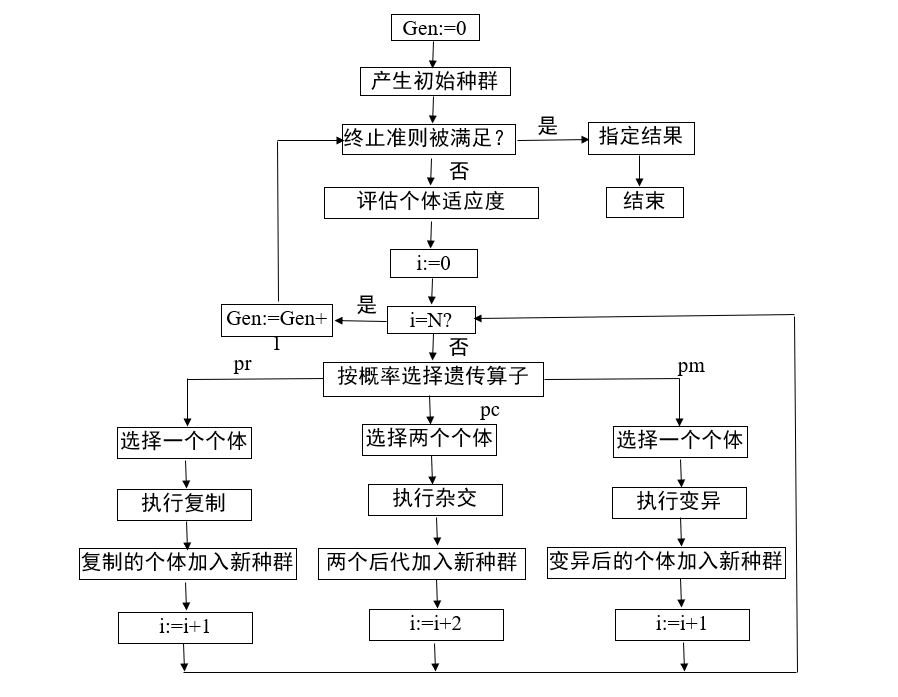
\includegraphics[scale=0.4]{../images/GP_framework.png}
\caption{遗传程序设计的流程图}
\label{fig:label}
\end{figure}
}

\frame{\frametitle{算法}
遗传程序设计的基本算法:	
	
(1)随机生成初始群体,其中个体是由表示问题的函数和终止符随机组合而成的计算机程序。
	
(2)循环执行下列各步直到满足终止准则为止:

I)运行群体中的每个计算机程序,并对其赋予适应度;

II)运行下面两个主要操作产生新的计算机程序群体:

\qquad i)把当前一代计算机程序复制成新一代计算机程序,被复制的个体依其适应度随机选定。

\qquad ii)随机选定双亲个体部位进行交叉操作产生新个体,双亲个体也依适应度随机选定。

(3)用结果标定法确定的程序被认为是运行的结果,它可能是一个正确(或近似)的问题答案。
}

\frame{\frametitle{关键}
遗传程序设计所需解决的关键问题:	
	
(1)程序的表示;

(2)程序好坏的评价标准;

(3)遗传算子的设计。
}

\frame{\frametitle{程序的表示}	
\parindent=19pt	
\renewcommand{\raggedright}{\leftskip=0pt \rightskip=0pt plus 0cm}
\raggedright
在遗传程序设计中,种群中的个体是计算机程序。为了程序表示的简单性和容易验证程序的句法,遗传程序设计用LISP语言来表示程序。

考虑一个简单的LISP程序,该程序简单地返回一个自然数n的平方:
	
>(defun square(n)(*nn))

SQUARE

下面是一个计算实数绝对值的LISP程序:

>(defun abs(x)(if(< x 0)(-x)(x)))

ABS

LISP程序的主体由类似于(*nn)和(if(< x 0)(-x)(x))的一些S-表达式所组成。

一般来说一个表示LISP程序的S-表达式通常由一些函数和端点组成。
}

\frame{\frametitle{程序的表示}	
\parindent=19pt	
\renewcommand{\raggedright}{\leftskip=0pt \rightskip=0pt plus 0cm}
\raggedright
构造LISP程序的S-表达式是以前缀表达式形式表示的。给定一个S-表达式,我们容易构造出它的语法树,而对该树进行先序遍历便可得到给定的S-表达式。
	
例如S-表达式(+12(if(> x 10)56))所对应的语法树如下图所示:

	\begin{figure}[ht]
		\centering	
		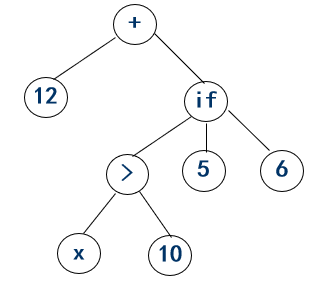
\includegraphics[scale=0.3]{../images/syntactic_tree.png}
		\caption{S-表达式的语法树}
		\label{fig:label}
	\end{figure}
	
在语法树中,树的外部结点(叶结点)分别用变量x和常量5,6,10,12来标记,这些变量和常量通常称为端点,而内部结点分别用函数+,>,IF来标记。
}

\frame{\frametitle{实现}
用遗传程序设计求解问题有以下五个基本步骤:
	\begin{itemize}		
		\item<1-> 选择端点集;
		\item<2-> 选择函数集;
		\item<3-> 确定适应函数;
		\item<4-> 确定控制参数;
		\item<5-> 确定指定结果的方法和终止程序运行的条件。
	\end{itemize}
}

\frame{\frametitle{选择端点集和函数集}
\renewcommand{\raggedright}{\leftskip=0pt \rightskip=0pt plus 0cm}
\raggedright
	\begin{itemize}		
		\item<1-> 在遗传程序设计中,计算机程序用LISP程序的语法树来表示。每一棵语法树的内部结点由一些函数构成,而叶结点由一些变量和常数构成。
		\item<2-> 对于一个给定的问题,首先要确定由所有可能求解该问题的程序所组成的程序空间S。由于LISP程序通常可以由一些简单的函数、变量和常数经过有限次运算和复合而生成。因此若要指定程序空间S,我们只要指定可以构成中程序的函数集和端点集。
		\item<3-> 函数集可以包含:
		
			<1> 算数运算 +,-,*,/等;
			
			<2> 数学函数 sin,cos,exp,log等;
			
			<3> 布尔运算 AND,OR,NOT等;
			
			<4> 条件运算 IF-THEN-ELSE等;
			
			<5> 循环运算 DO-UNTIL,FOR,WHILE等。
		\item<4-> 端点集通常由变量和常量组成。
	\end{itemize}
}

\frame{\frametitle{初始化}
	\renewcommand{\raggedright}{\leftskip=0pt \rightskip=0pt plus 0cm}
	\raggedright
	\begin{itemize}		
		\item<1-> 假设问题的端点集和函数集分别为T和F。
		\item<2-> 初始种群中的每个S-表达式,即每棵树,可按以下步骤产生:
		
			<1> 首先建立一个根结点,从函数集F中随机地选择一个函数作为根结点的标记;
		
			<2> 每当树中的一个结点被标记为函数集F中的一个函数$f$后,则为该结点建立$z(f)$个儿子结点,而每个儿子结点的标记从$C=F \bigcup T$中随机地选取;
		
			<3> 每当树中一个结点被标记为端点集T中的一个元素时,则该结点成为树的一个叶结点;
		
			<4> 如此反复进行,直到所有结点都被标记。
	\end{itemize}
}

\frame{\frametitle{初始化}
	\renewcommand{\raggedright}{\leftskip=0pt \rightskip=0pt plus 0cm}
	\raggedright
	\begin{itemize}		
		\item<1-> 假定F=\{+,-,*,/\},T=\{a,b,c,d\}。下面给出了建立一棵树结构的过程:
			\begin{figure}[ht]
			\centering	
			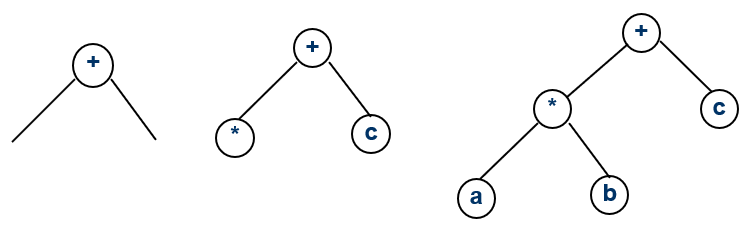
\includegraphics[scale=0.5]{../images/build_tree.png}
			\caption{语法树的构建}
			\label{fig:label}
			\end{figure}
	\end{itemize}
}

\frame{\frametitle{适应函数}
	\parindent=19pt	
	\renewcommand{\raggedright}{\leftskip=0pt \rightskip=0pt plus 0cm}
	\raggedright
	适应性函数是遗传算法和遗传程序设计得以实现的关键因素,是评价个体好坏的定量表述,决定着演化过程中群体选择复制及群体整体性的质量。

	与其它演化算法相同,在遗传程序设计中,个体的适应性函数值是判断个体的质量的唯一办法。
	
	个体适应性函数值的计算方法是问题相关的,有多种方式度量个体的适应性函数值,有些方法是明确的,有些方法是隐含的。
	
	例如,若个体是下列程序:
		\begin{figure}[ht]
		\centering	
		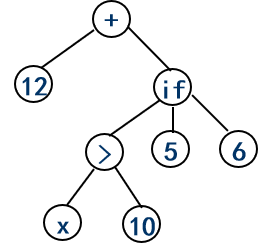
\includegraphics[scale=0.3]{../images/program.png}
		\caption{程序示例}
		\label{fig:label}
		\end{figure}
}

\frame{\frametitle{适应函数}
	\renewcommand{\raggedright}{\leftskip=0pt \rightskip=0pt plus 0cm}
	\raggedright
	评估该程序好坏的一种方法是:
	
	(1) 建立一个样本集$\{(x_{i},y_{i})|i=1,2,\Lambda,s\}$,其中$y_{i}$是当变量x取值为$x_{i}$时的期望输出;

	(2) 当$x=x_{i}(i=1,2,\Lambda,s)$时,运行该程序得到输出$z_{i}$;

     (3) 计算所得到的输出与期望输出之间的误差的绝对值之和$e=\Sigma|z_{i}-y_{i}|$;

     (4) 最后,用e作为该个体的适应性函数值。显然,适应性函数值越小,个体越好。
	
	\parindent=19pt	
	若个体是判定树,则判定树的分类准确率可以作为个体的适应性函数值。若个体是游戏策略,则游戏策略与其它策略对奕时取胜的次数可以作为个体的适应性函数值。
}

\frame{\frametitle{适应函数}
	\renewcommand{\raggedright}{\leftskip=0pt \rightskip=0pt plus 0cm}
	\raggedright
	个体适应性函数值有以下几种形式:
	
	(1) 原始适应性函数值;
	
     原始适应性函数值是以问题本身的自然术语叙述的适应性函数值度量。

     (2) 标准适应性函数值;
	
     标准适应性函数值对原始适应性函数值作简单变换,使得标准适应性函数值越小,个体越好。

     (3) 调整适应性函数值;

     调整适应性函数值$\epsilon(0,1]$。调整适应性函数值越大,个体越好。

     (4) 正规化适应性函数值。
		
	\parindent=19pt	
	正规化适应性函数值$\epsilon[0,1]$,在基于适应性函数值比例的选择策略中可直接用作选择概率。
}

\frame{\frametitle{适应函数}
	\renewcommand{\raggedright}{\leftskip=0pt \rightskip=0pt plus 0cm}
	\raggedright
	设计适应性函数,一般有以下几个步骤:
	
	(1) 原始适应性函数;
	
     按照目标函数的计算方法直接计算原始适应性函数值。

     (2) 标准化适应性函数;
	
     将得出的原始适应性函数表述为标准适应性函数。

     (3) 优化调整适应性函数;

     调整最优个体与次优个体的微小差别。

     (4) 正规化适应性函数。
		
	正规化(归一化)已优化调整的适应性函数值。
}

\frame{\frametitle{父体选择策略}
	\renewcommand{\raggedright}{\leftskip=0pt \rightskip=0pt plus 0cm}
	\raggedright	
	(1) 通常,遗传程序设计使用基于适应性函数值比例的选择策略。
	
	(2) 若种群规模在1000以上,则经常使用一种贪婪过度选择策略。
	
	(3)该策略首先将种群中的个体按适应性函数值排序,然后将种群中的个体分为两部分。第一部分包含种群$x\%$的最好个体,另一部分包含其它$(1-x\%)$的个体。当进行父体选择时,80\%的选择在第一部分中进行,20\%的选择在第二部分中进行。x的取值以来于种群规模,通常通过实验确定。
		\begin{figure}[ht]
			\centering	
			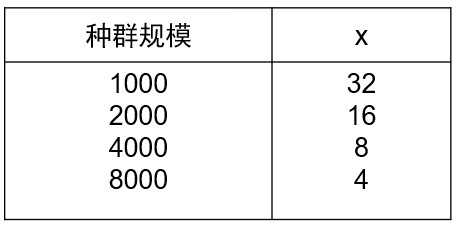
\includegraphics[scale=0.3]{../images/x_value.png}
			\caption{x的取值}
			\label{fig:label}
		\end{figure}
	
	\parindent=19pt	
	从上表可以看出,随着种群规模的增加,x不断减小,选择压力逐步增大。
}

\frame{\frametitle{遗传算子}
	\parindent=19pt
	\renewcommand{\raggedright}{\leftskip=0pt \rightskip=0pt plus 0cm}
	\raggedright	
	遗传程序设计中的遗传算子主要有复制、杂交和变异。变异算子的作用不及遗传算法中重要。
	
	(1) 复制
	
	复制算子首先按照某种基于适应性函数值比例的选择策略从种群中选择一个个体,然后将该个体不加改变地复制到下一代种群。
	
	(2) 杂交

    杂交算子分别从两个父体中随机地选择一个杂交点,然后交换父体中以杂交点为根结点的子树产生两个后代。
}

\frame{\frametitle{遗传算子}
	\renewcommand{\raggedright}{\leftskip=0pt \rightskip=0pt plus 0cm}
	\raggedright	
 	\begin{figure}[ht]
		\centering	
		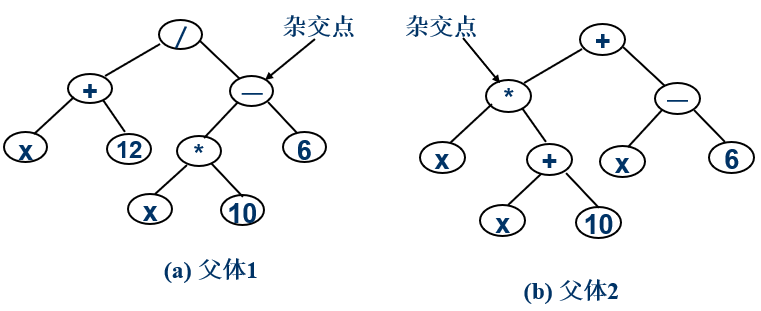
\includegraphics[scale=0.35]{../images/Hybridization1.png}
		\caption{杂交前}
		\label{fig:label}
	\end{figure}
     \begin{figure}[ht]
		\centering	
		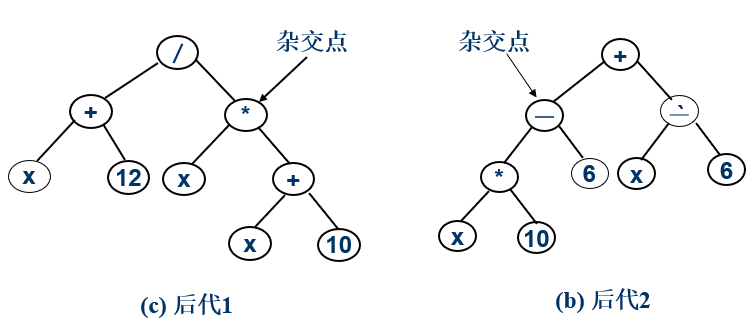
\includegraphics[scale=0.35]{../images/Hybridization2.png}
		\caption{杂交后}
		\label{fig:label}
	\end{figure}
}

\frame{\frametitle{遗传算子}
    \renewcommand{\raggedright}{\leftskip=0pt \rightskip=0pt plus 0cm}
	\raggedright	
    (3) 变异
    
    \parindent=19pt
    变异算子首先在父体中随机地选择一个结点,然后删除以该结点为根结点的子树,并在该结点处插入一个随机生成的子树。
        \begin{figure}[ht]
			\centering	
			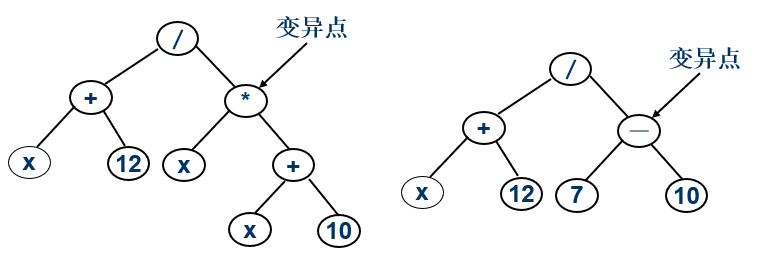
\includegraphics[scale=0.5]{../images/variation.png}
			\caption{变异}
			\label{fig:label}
		\end{figure}	
}

\frame{\frametitle{应用}
	\begin{itemize}
		\item<1-> 预测和分类:使用历史数据库来预测新事例。
		\item<2-> 符号压缩:发现各变量间的隐含关系。
		\item<3-> 机器人:控制机器人行为,使其对环境做出反应。
		\item<4-> 人工生命:用计算机模拟生物的自然进化或发现规律。
		\item<5-> 神经网络设计“设计神经网络结构、发现学习规则和相关权值,以使神经网络完成指定的任务。
		\item<6-> 图像和信号处理:图像识别、图像恢复、图像和声音的压缩等。
		\item<7-> 多Agent系统的自动设计:多个Agent协作共同处理实际问题。
		\item<8-> 游戏策略:发现一个策略打败对手。
		\item<9-> 艺术:声音、三维图像的生成、计算机动画等。
	\end{itemize}
}

\frame{\frametitle{应用实例1}
	\renewcommand{\raggedright}{\leftskip=0pt \rightskip=0pt plus 0cm}
	\raggedright	
	\begin{figure}[ht]
	\centering	
	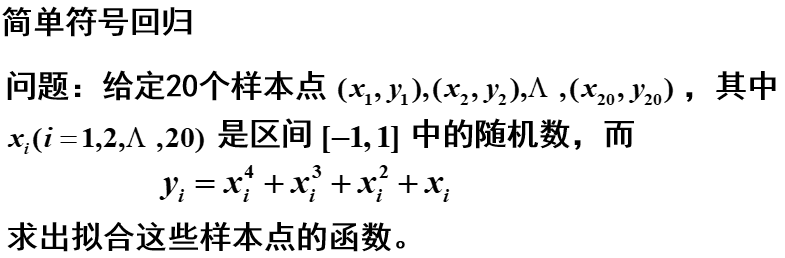
\includegraphics[scale=0.5]{../images/question.png}
	\end{figure}
}

\frame{\frametitle{应用实例1}
	\renewcommand{\raggedright}{\leftskip=0pt \rightskip=0pt plus 0cm}
	\raggedright	
	\begin{figure}[ht]
		\centering	
		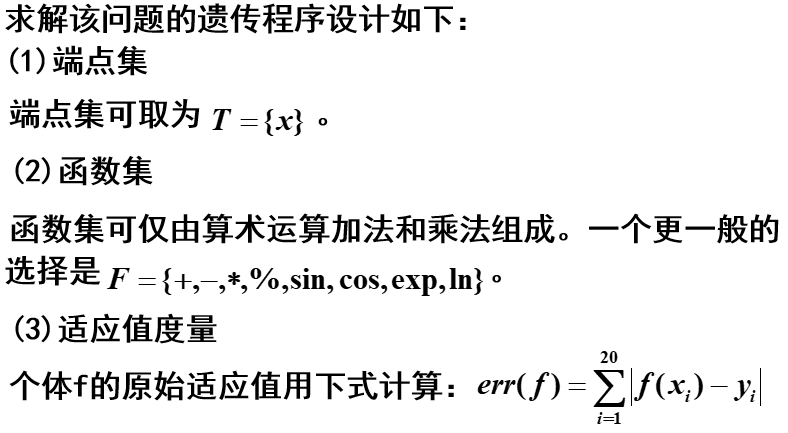
\includegraphics[scale=0.5]{../images/answer1.png}
	\end{figure}
}

\frame{\frametitle{应用实例1}
	\renewcommand{\raggedright}{\leftskip=0pt \rightskip=0pt plus 0cm}
	\raggedright	
	\begin{figure}[ht]
		\centering	
		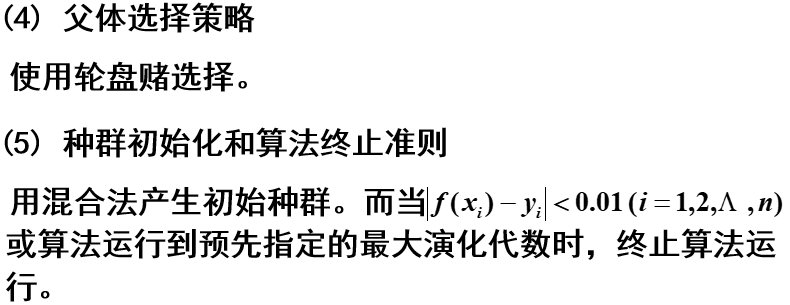
\includegraphics[scale=0.5]{../images/answer2.png}
	\end{figure}
}

\frame{\frametitle{应用实例1}
	\renewcommand{\raggedright}{\leftskip=0pt \rightskip=0pt plus 0cm}
	\raggedright	
	\begin{figure}[ht]
		\centering	
		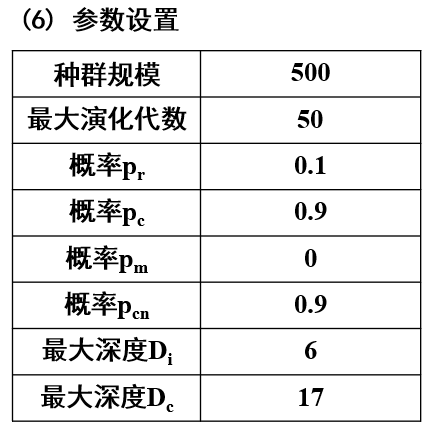
\includegraphics[scale=0.5]{../images/answer3.png}
	\end{figure}
}

\frame{\frametitle{应用实例1}
	\renewcommand{\raggedright}{\leftskip=0pt \rightskip=0pt plus 0cm}
	\raggedright	
	\begin{figure}[ht]
		\centering	
		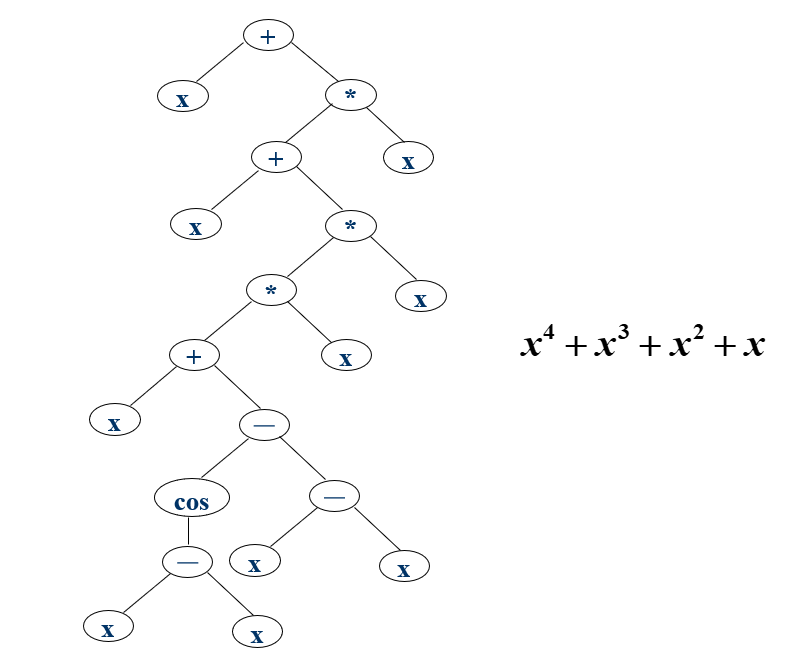
\includegraphics[scale=0.45]{../images/answer4.png}
	\end{figure}
}

\frame{\frametitle{应用实例2}
	\parindent=19pt
	\renewcommand{\raggedright}{\leftskip=0pt \rightskip=0pt plus 0cm}
	\raggedright	
	问题:给定数学表达式cos(2x),我们希望发现与cos(2x)恒等的数学表达式。
	
	将该问题视为一个符号回归问题。通过在某个区间内抽取一个随机样本,并计算给定函数在该样本的函数值,这样形成一组样本点,对所形成的样本点作符号回归。
}

\frame{\frametitle{应用实例2}
	\renewcommand{\raggedright}{\leftskip=0pt \rightskip=0pt plus 0cm}
	\raggedright	
	\begin{figure}[ht]
		\centering	
		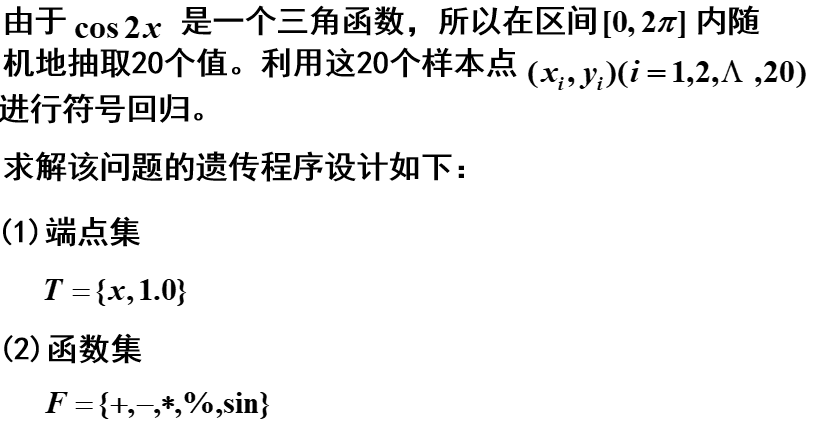
\includegraphics[scale=0.5]{../images/answer11.png}
	\end{figure}
}

\frame{\frametitle{应用实例2}
	\renewcommand{\raggedright}{\leftskip=0pt \rightskip=0pt plus 0cm}
	\raggedright	
	\begin{figure}[ht]
		\centering	
		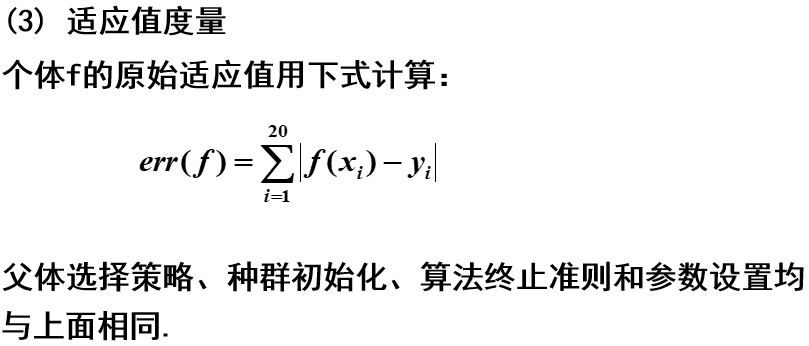
\includegraphics[scale=0.5]{../images/answer22.png}
	\end{figure}
}

\frame{\frametitle{应用实例2}
	\renewcommand{\raggedright}{\leftskip=0pt \rightskip=0pt plus 0cm}
	\raggedright	
	\begin{figure}[ht]
		\centering	
		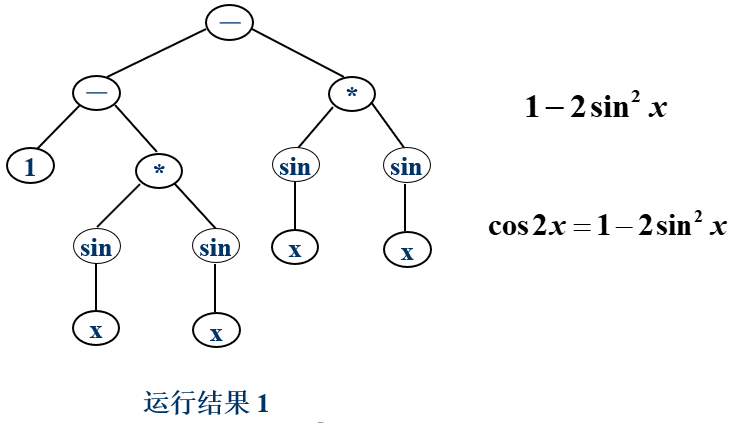
\includegraphics[scale=0.5]{../images/answer33.png}
	\end{figure}
}

\frame{\frametitle{应用实例2}
	\renewcommand{\raggedright}{\leftskip=0pt \rightskip=0pt plus 0cm}
	\raggedright	
	\begin{figure}[ht]
		\centering	
		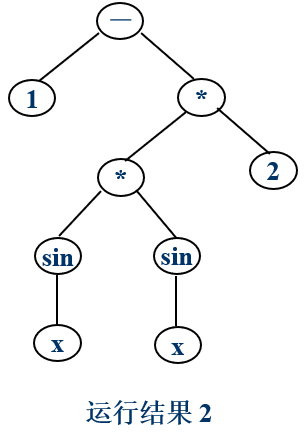
\includegraphics[scale=0.5]{../images/answer44.png}
	\end{figure}
}

\frame{\frametitle{应用实例2}
	\renewcommand{\raggedright}{\leftskip=0pt \rightskip=0pt plus 0cm}
	\raggedright	
	\begin{figure}[ht]
		\centering	
		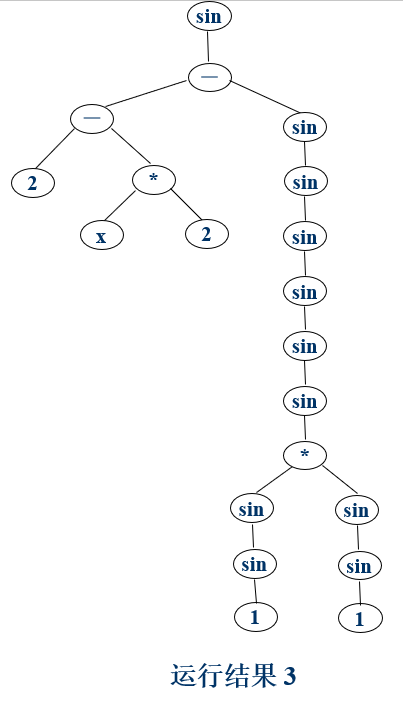
\includegraphics[scale=0.45]{../images/answer55.png}
	\end{figure}
}

\frame{\frametitle{应用实例2}
	\renewcommand{\raggedright}{\leftskip=0pt \rightskip=0pt plus 0cm}
	\raggedright	
	\begin{figure}[ht]
		\centering	
		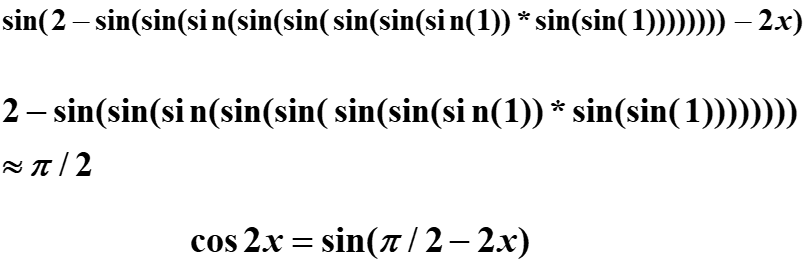
\includegraphics[scale=0.5]{../images/answer66.png}
	\end{figure}
}

\frame{\frametitle{改进}
	\parindent=19pt	
	\renewcommand{\raggedright}{\leftskip=0pt \rightskip=0pt plus 0cm}
	\raggedright
	遗传程序设计作为一种优化算法具有不需要先验性假设而可以进行全局搜索和进化最终得到最优解的特点,近年来人们在研究使用这种算法的过程中,也针对实际应用对其作了一些相应的改进:
	
	遗传程序设计主要处理树状具有分层结构的程序,在实际编程中多采用LISP语言实现。LISP语言由于缺乏统一的标准和方便的对外接口,作为一种解释语言运行速度较慢,可以采用几种具有不同数据类型的语言如PROL0G和C语言来加速程序进化的进程。
	
	传统的遗传程序设计限制少、搜索速度慢,可以用定向的非周期图(DAG)取代树和森林来存储程序群体,或针对子树进行改进,以节省程序的运行时间和空间。
	
	在算法方面,遗传程序设计可以与包括遗传算法、神经网络和模拟退火等的其他优化方法相结合,以得到更好的应用。
}

%end

%
% GNU, Yi Zhang, 2018
%

\section{多种群协同进化}\renewcommand{\baselinestretch}{1.5} \normalsize:

\frame{ \frametitle{定义}
	\setlength{\parindent}{2em}
	协同演化算法(coevolutionary algorithm,CEA)通过构造两个或多个种群,
	建立它们之间的竞争或合作关系,多个种群通过相互作用来提高各自性能,
	适应复杂系统的动态演化环境, 以达到种群优化的目的.
}

\frame{ \frametitle{背景}
	\setlength{\parindent}{2em}
	演化算法,基于个体自身适应度:\\
	~~1.~未成熟收敛\\
	~~2.~收敛速度慢\\
	~\\
	~\\
	协同演化算法,一个个体适应度在与其他个体(同种群个体,不同种群个体)的交互过程中计算.
}

\frame{\frametitle{framework}
	\begin{figure}[ht]
		\centering	
		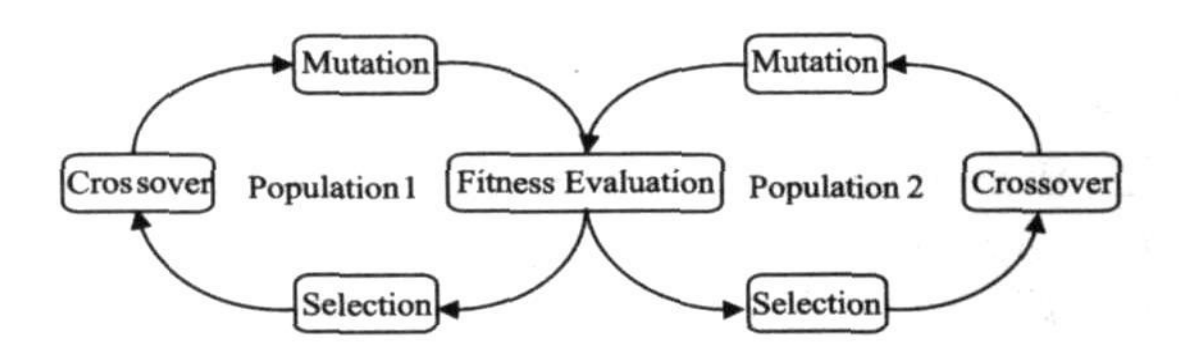
\includegraphics[scale=0.25]{../images/cc_framework.png}
		\caption{the framework of CEA}
		\label{fig:label}
	\end{figure}
}

\frame{ \frametitle{应用}
	\setlength{\parindent}{5em}
	1> ~~  函数优化\\
	2> ~~  多目标优化\\
	3> ~~  分类\\
	4> ~~  图像分割\\
	5> ~~  神经网络设计\\
	6> ~~  工程设计
}

\frame{ \frametitle{ 分类 }
	\setlength{\parindent}{4em}
	>> ~~  合作型协同进化算法(Coop-CEA)\\
	~\\
	~\\
	>> ~~  竞争型协同进化算法(Comp-CEA)\\
}

%合作型协同进化算法
\frame{ \frametitle{ Coop-CEA }
	\setlength{\parindent}{2em}
	Coop-CEA使用分治策略将演化算法(EA)应用于大型复杂问题的中.
	原始问题被分解成更小的模块,并且每个模块都被分配到一个物种。
	这些物种大多分开进化,唯一的合作发生在适应性评估期间。
}


\frame{ \frametitle{ Coop-CEA一般框架 }
	\begin{itemize}
		\item<1->  Decompose an objective vector into m low-dimensional subcomponents.
		\item<2->  Set i = 1 to start a new cycle.
		\item<3->  Optimize the ith subcomponent with a certain EA for a predefined number of fitness evaluations (FEs).
		\item<4->  If i < m then i ++, and go to Step 3.
		\item<5->  Stop if halting criteria are satisfied; otherwise go to Step 2 for the next cycle.
	\end{itemize}
}

\frame{ \frametitle{ Coop-CEA任务分解 }
	\setlength{\parindent}{2em}
	Coop-CEA中,每个个体只表示解的一部分,每个种群求一个部分解.把多个自种群的最终解连接起来就是Coop-CEA的解.\\
	~\\
	任务分解:\\
	1.~随机分解:随机选择基因的顺序\\
	2.~扰动:使用扰动决策变量尝试对变量进行分组\\
	3.~模型构建:基于个体数量的概率模型
}

\frame{ \frametitle{ Coop-CEA适应度计算 }
	\setlength{\parindent}{2em}
	Coop-CEA中,个体的适应度表现为与其他各种群的合作能力\\
	从其它的每一个子群体接收若干“合作者”来同该个体合作,一起组成若干完整的解。求得的适应度中的最佳值作为所求个体的适应度。\\
	~\\
	合作者可以随机选择,也可以选择种群中最佳个体\\
	合作者可多可少
}

%竞争型协同进化算法
\frame{ \frametitle{ Comp-CEA }
	\setlength{\parindent}{2em}
	竞争型协同进化的核心思想就是物种间的相互作用,这种相互作用的结果使得物种获得进化的动力\\
	~\\
	一个种群中的个体适应度是由其他种群的个体的一系列竞争作用来决定的协同进化
}

\frame{ \frametitle{ Comp-CEA workfow }
	\setlength{\parindent}{2em}
	BEGIN\\
	~Initialize Pop1, Pop2\\
	~Let Pop1 serve as learner\\
	~Select the set of evaluators(E) from Pop2\\
	WHILE( not termination )\\
	~~~~Evaluation(learner)\\
	~~~~Selection(learner)\\
	~~~~Crossover(learner)\\
	~~~~Mutation(learner)\\
	~~~~Interehange the individuals in Pop1 and Pop2\\
	~~~~Select the set of evaluators form Pop2\\
	END
}

\frame{ \frametitle{ Comp-CEA适应度计算 }
	\setlength{\parindent}{2em}
	竞争适应度:一个种群的个体对对手竞争力的大小\\
	~\\
	~\\
	种群适应度:一个种群相对其他种群的竞争力的大小
}

\frame{ \frametitle{ Comp-CEA适应度计算 }
	\setlength{\parindent}{2em}
	简单竞争适应度\\
	\begin{equation}
		\forall i \in L \Rightarrow CF_i = \sum_{j \in E,\;i\;defeat\;j}1
	\end{equation}\\
	共享竞争适应度\\
	\begin{equation}
		\forall j \in E \Rightarrow N_j = \sum_{k \in L,\;k\;defeat\;j}1
	\end{equation}
	\begin{equation}
		\forall i \in L \Rightarrow CF_i = \sum_{j \in E,\;i\;defeat\;j}\frac{1}{N_j}
	\end{equation}\\
	~\\
	L:学习者~~~~~E:评价者
	
}

\frame{ \frametitle{ Comp-CEA评价者选取 }
	\setlength{\parindent}{2em}
	具有相同染色体的个体,可能由于临时对手的不同,得到不同的适应度\\
	~\\
	~~~随机配对\\
	~~~随机选定多个临时对手\\
	~~~穷举
}

%end
%
% GNU courseware, Zhang Jiadong, 2018
%

\section{差分进化}\fontsize{12pt}{12pt}\selectfont

\subsection{定义}
\begin{frame}{定义}
	{\bf差分进化}是一种基于群体智能的全局优化方法,其主要通过种群内个体之间的协同合作
		和相互竞争来产生群体智能,进一步指导进化过程的全局搜索。
\end{frame}

\subsection{算法思想}
\begin{frame}{算法思想}
	\begin{figure}
		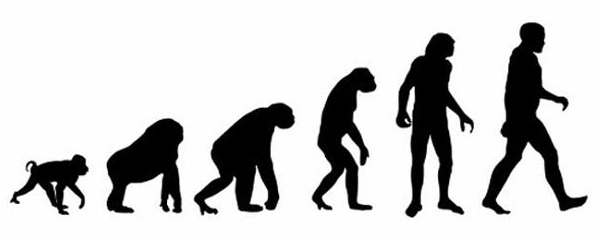
\includegraphics [width =1.0\textwidth]{../images/evolution.png}
	\end{figure}
	通过种群之间的\textbf{个体差异}和\textbf{优胜劣汰}的竞争策略产生新的个体,最终使种群接近或达到全局最优解。
\end{frame}

\subsection{算法框架}
\begin{frame}{算法框架}\small
	\begin{figure}
		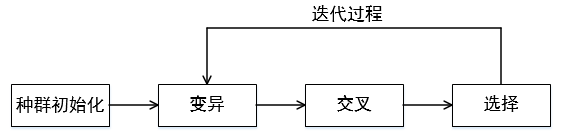
\includegraphics [width =1.0\textwidth]{../images/framework.png}
		\vspace{-1.2cm}
	\end{figure}
	\begin{itemize}
		\item {\bf 种群初始化}在解空间中随机、均匀地产生$M$个个体,每个个体由$n$个染色体组成,作为第$0$代种群,标记为
		\begin{equation*}
			\begin{split}
				X_i(0)=&\left(x_{i,1}(0),x_{i,2}(0),\cdots,x_{i,n}(0)\right)\\
				& i=1,2,\cdots,M
			\end{split}
		\end{equation*}
		\item {\bf 变异、交叉、选择 }三步操作迭代执行,直到算法收敛。第$g$次迭代的第$i$个个体标记为
		\begin{equation*}
			\begin{split}
				X_i(g)=&\left(x_{i,1}(g),x_{i,2}(g),\cdots,x_{i,n}(g)\right)\\
				& i=1,2,\cdots,M
			\end{split}
		\end{equation*}
	\end{itemize}
\end{frame}

\begin{frame}{种群初始化}
	在$n$维空间里随机产生满足约束条件的$M$个染色体,第$i$个染色体的第$j$个维取值方式如下(rand(0,1)产生0到1的均匀分布的随机数) :
	\begin{equation*}
		\begin{split}
			x_{i,j}(0) &= L_j + rand(0,1)\left(U_j-L_j\right)\\
			& i = 1,2,\cdots,M\\
			& j = 1,2,\cdots,n\\
		\end{split}
	\end{equation*}
\end{frame}

\begin{frame}{变异算子}
	在第$g$次迭代中,对个体$X_i(g)=\left(x_{i,1}(g),x_{i,2}(g),\cdots,x_{i,n}(g)\right)$,从种群中随机选择$3$个个体 $X_{p1}(g),X_{p2}(g),X_{p3}(g)$,且$ p1 \neq p2 \neq p3\neq i$, 则
	$$H_{i}(g) = X_{p1}(g)+ F\cdot\left(X_{p2}(g)-X_{p3}(g)\right)$$
	% 其中$\Delta_{p2,p3}(g)=X_{p2}(g)-X_{p3}(g)$是差分向量;$F$是缩放因子,用于控制差分向量的影响力.
	\begin{figure}
		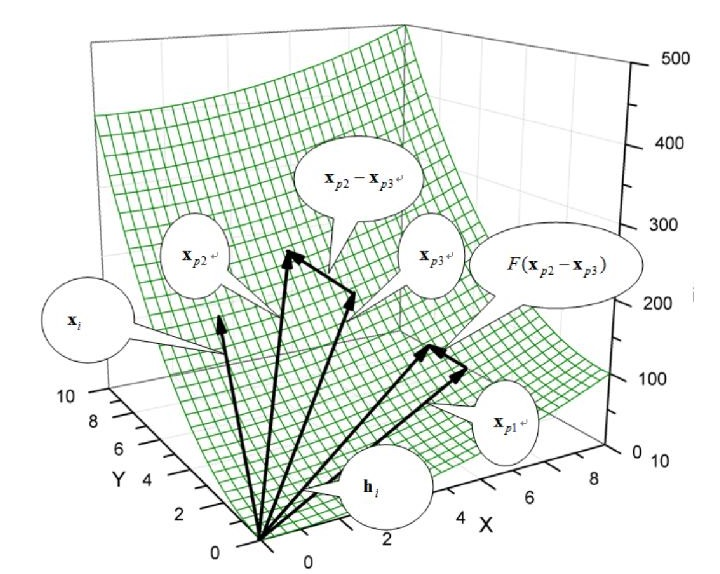
\includegraphics [width =0.55\textwidth]{../images/mutation.png}
	\end{figure}
\end{frame}

\begin{frame}{交叉算子}
	交叉操作可以增加种群的多样性,方法如下:
	$$
	v_{i,j}(g)=
	\begin{cases}
	h_{i,j}(g), rand(0,1)\le cr\\
	x_{i,j}(g), else
	\end{cases}
	$$
	其中$cr\in[0,1]$为交叉概率,$rand(0,1)$是$[0,1]$上服从均匀分布的随机数。

	\begin{figure}
		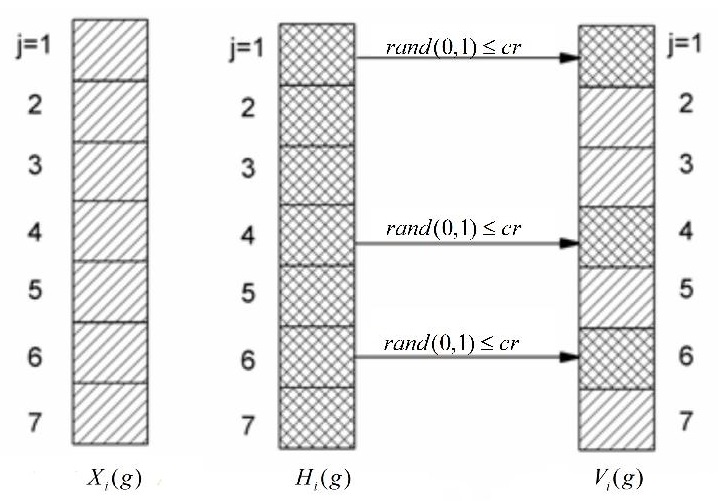
\includegraphics [width =0.55\textwidth]{../images/cross.png}
	\end{figure}
\end{frame}

\begin{frame}{选择算子}
首先查看根据评价函数选择$V_i(g)$ 或 $X_i(g)$ 作为$X_i(g+1)$
$$
	X_i(g+1) =
	\begin{cases}
	V_i(g),\qquad \mathrm{if} \quad f(V_i(g))< f(X_i(g))\\
	X_i(g),\qquad else
	\end{cases}
$$

可以看出:
	\begin{itemize}
		\item 对每个个体,$X_i(g+1)$要好于或持平$X_i(g)$。
		\item 肯定会收敛于最优点(可能是局部最优)。
		\item {\bf 变异、交叉} 操作有助于突破局部最优到达全局最优。
	\end{itemize}
\end{frame}

\subsection{应用实例}
	\begin{frame}{差分进化算法寻找函数最优解}
	定义关于参数$x, y$的函数,函数图像如左图所示
	$$f(x,y)=-20e^{-0.2\sqrt{\frac{x^2+y^2}{2}}}-e^{\frac{\cos2\pi x+\cos2\pi y}{2}}+20+e$$
	用差分进化算法求解,效果如右图所示(参数设置:$N=20, F=0.5, cr=0.5$,迭代次数 $T=300$)
	\begin{columns}
		\begin{column}{0.45\textwidth}
			\begin{figure}
				\vspace{-0.8cm}
				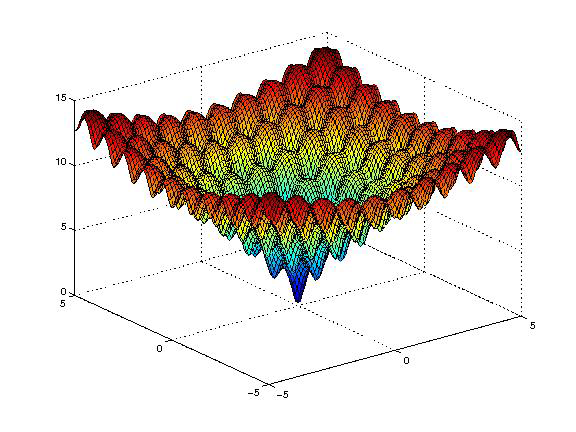
\includegraphics [width =2.0in]{../images/function.png}
			\end{figure}
		\end{column}
		\begin{column}{0.55\textwidth}
			\begin{figure}
				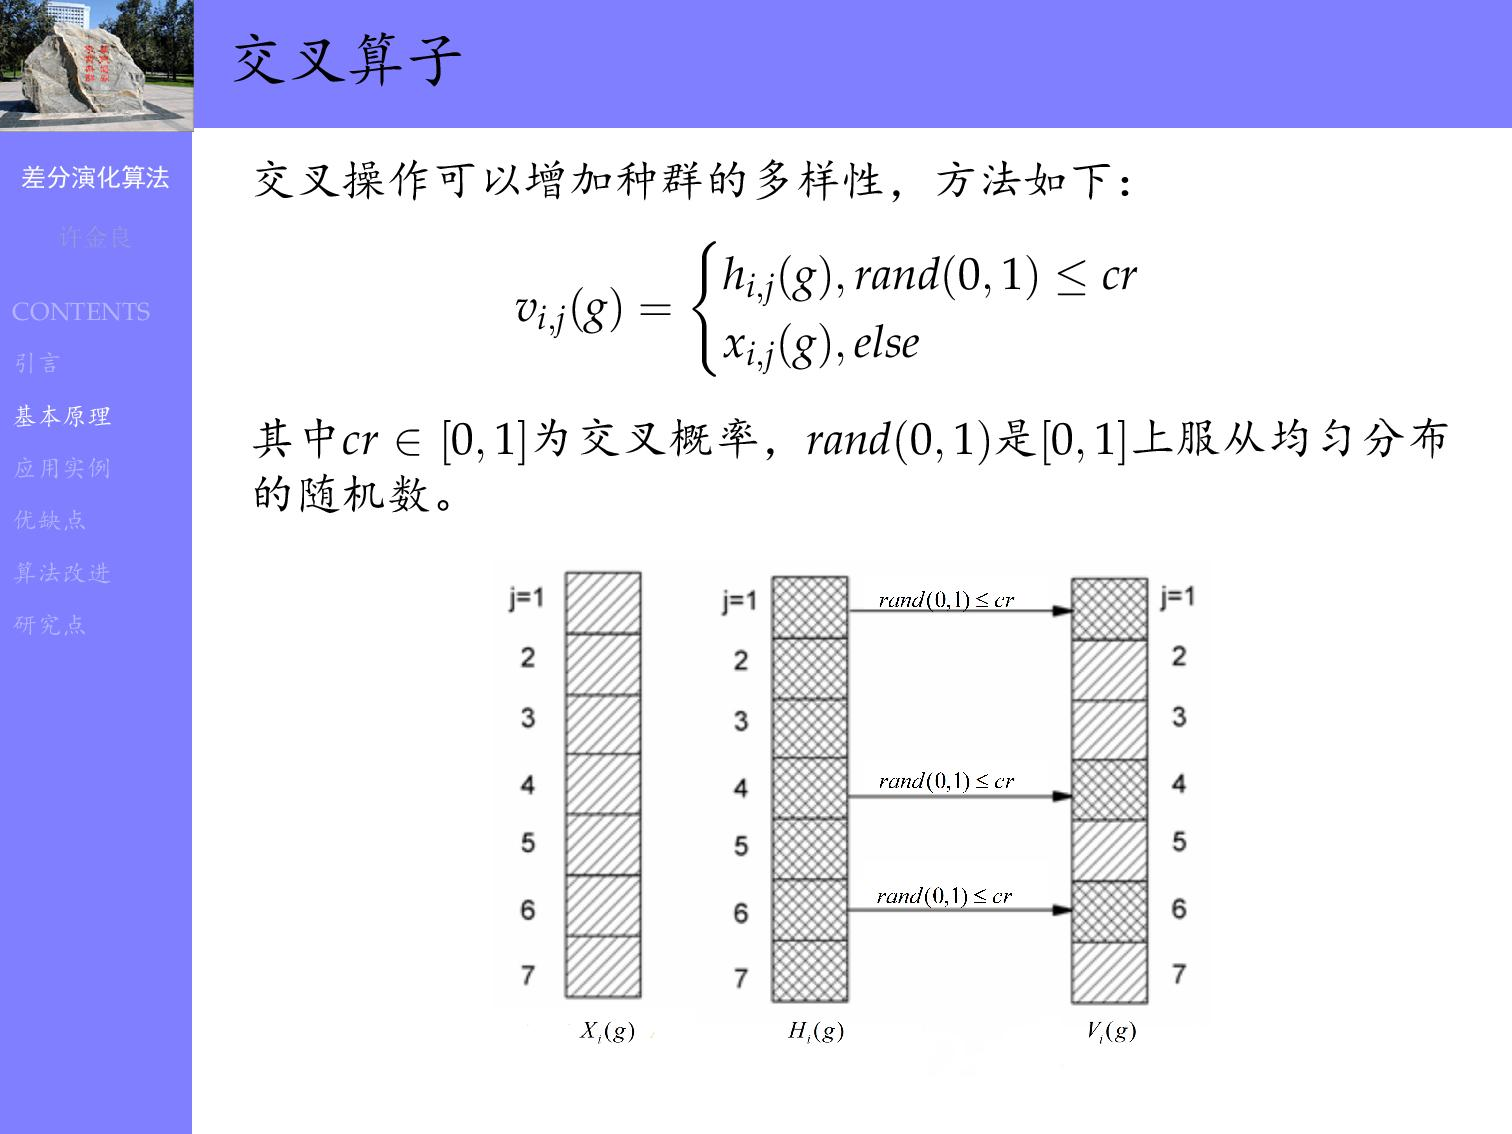
\includegraphics [width =2.0in]{../images/curve.png}
			\end{figure}
		\end{column}
	\end{columns}
\end{frame}

\subsection{优缺点}
\begin{frame}{优缺点}
和其他进化算法相比,差分进化算法具有以下优点:
	\begin{enumerate}
		\item 在非凸、多峰、非线性、连续不可微函数优化问题上表现出极强的稳健性。
		\item 收敛速度快。
		\item 操作简单,容易实现。
	\end{enumerate}
	缺点:
	\begin{enumerate}
		\item 算法后期个体间差异逐渐缩小,收敛速度慢,容易陷入局部最优。
		\item 控制参数和学习策略对算法性能有着重要的影响,并且高度依赖于优化问题的本质。
		\item 有时需要过多的迭代才能搜索到全局最优。
	\end{enumerate}
\end{frame}


\subsection{算法改进}
\subsubsection{参数控制}

\begin{frame}{参数的选取}
%参数选择主要涉及群体规模$M$,缩放因子$F$,以及交叉概率$cr$的设定\footnote{
%各研究人员得到的经验参数值往往不一致,甚至相互矛盾,所以要具体问题具体分析。}
	\begin{itemize}
		\item $M$:一般介于$5\times n$与$10\times n$之间,但不能少于$4$,否则变异算子无法进行;
		\item $F$:一般在$[0,2]$之间选择,通常取$0.5$;
		\item $cr$:一般在$[0,1]$之间选择,比较好的选择应在$0.3$左右。$cr$取值偏大,收敛速度会加快,但易发生早熟现象。
	\end{itemize}
\end{frame}

\begin{frame}{参数的自适应调整($F$)}
	将变异算子中随机选择的三个个体进行从优到劣的排序,得到$X_b,X_m,X_w$,对应适应度$f_b,f_m,f_w$,则变异算子改为:
	$$V_i=X_b+F_i\left(X_m-X_w\right)$$
	同时,$F$的取值根据生成差分向量的两个个体自适应变化,平衡全局搜索和局部搜索之间的矛盾。
	$$F_i = F_l +\left(F_u-F_l\right)\frac{f_m-f_b}{f_w-f_b}$$
	其中,$$F_l=0.1,F_u=0.9$$
\end{frame}

\begin{frame}{参数的自适应调整($cr$)}
	对于适应度好的解,取较小的$cr$,使得该解进入下一代的机会增大;
	对于适应度差的解,则取交大的$cr$,加快改变该个体的结构,使该解被淘汰掉。
	$$
	cr_i =
	\begin{cases}
		cr_l+\left(cr_u-cr_l\right)\frac{f_i-f_{min}}{f_{max}-f_{min}}  \qquad \mathrm{if} \quad f_i>\bar{f} \\
		cr_l \qquad\qquad \qquad \qquad \qquad \quad \mathrm{if}\quad f_i<\bar{f}
	\end{cases}
	$$
	其中 $f_i$是个体$X_i$的适应度,$f_{min}$和$f_{max}$分别是当前种群中最差和最优个体的适应度,
	$\bar{f}$是当前种群适应度平均值,$cr_l$和$cr_u$分别是$cr$的下限和上限,一般$cr_l=0.1,cr_u=0.6$。
\end{frame}

\subsubsection{变异策略}
\begin{frame}{变异策略}
	变异策略表示为$DE/a/b$,其中$a$表明被变异个体的选择方式,$b$表明差向量的个数。
		\begin{enumerate}
		\item {\bf DE/rand/1:}\\\qquad$V_i = X_{p1}+F\left(X_{p2}-X_{p3}\right)$
		\item {\bf DE/best/1:}\\\qquad$V_i = X_{best}+F\left(X_{p1}-X_{p2}\right)$
		\item {\bf DE/current to best/1:}\\\qquad$V_i = X_{i}+F\left(X_{best}-X_{i}\right)+F\left(X_{p1}-X_{p2}\right)$
		\item {\bf DE/best/2:}\\\qquad$V_i=X_{best}+F\left(X_{p1}-X_{p2}\right)+F\left(X_{p3}-X_{p4}\right)$
		\item {\bf DE/rand/2:}\\\qquad$V_i = X_{p1}+F\left(X_{p2}-X_{p3}\right)+F\left(X_{p4}-X_{p5}\right)$
	\end{enumerate}
\end{frame}

% \end{CJK*}
% \end{document}

%end

\begin{frame}\fontsize{30pt}{30pt}\selectfont
	\begin{center}
		谢谢!
	\end{center}
\end{frame}

\iffalse

\section{Title formats}

\begin{frame}{Metropolis title formats}
	\themename supports 4 different title formats:
	\begin{itemize}
		\item Regular
		\item \textsc{Small caps}
		\item \textsc{all small caps}
		\item ALL CAPS
	\end{itemize}
	They can either be set at once for every title type or individually.
\end{frame}

{
    \metroset{titleformat frame=smallcaps}
\begin{frame}{Small caps}
	This frame uses the \texttt{smallcaps} title format.

	\begin{alertblock}{Potential Problems}
		Be aware that not every font supports small caps. If for example you typeset your presentation with pdfTeX and the Computer Modern Sans Serif font, every text in small caps will be typeset with the Computer Modern Serif font instead.
	\end{alertblock}
\end{frame}
}

{
\metroset{titleformat frame=allsmallcaps}
\begin{frame}{All small caps}
	This frame uses the \texttt{allsmallcaps} title format.

	\begin{alertblock}{Potential problems}
		As this title format also uses small caps you face the same problems as with the \texttt{smallcaps} title format. Additionally this format can cause some other problems. Please refer to the documentation if you consider using it.

		As a rule of thumb: just use it for plaintext-only titles.
	\end{alertblock}
\end{frame}
}

{
\metroset{titleformat frame=allcaps}
\begin{frame}{All caps}
	This frame uses the \texttt{allcaps} title format.

	\begin{alertblock}{Potential Problems}
		This title format is not as problematic as the \texttt{allsmallcaps} format, but basically suffers from the same deficiencies. So please have a look at the documentation if you want to use it.
	\end{alertblock}
\end{frame}
}

\section{Elements}

\begin{frame}[fragile]{Typography}
      \begin{verbatim}The theme provides sensible defaults to
\emph{emphasize} text, \alert{accent} parts
or show \textbf{bold} results.\end{verbatim}

  \begin{center}becomes\end{center}

  The theme provides sensible defaults to \emph{emphasize} text,
  \alert{accent} parts or show \textbf{bold} results.
\end{frame}

\begin{frame}{Font feature test}
  \begin{itemize}
    \item Regular
    \item \textit{Italic}
    \item \textsc{Small Caps}
    \item \textbf{Bold}
    \item \textbf{\textit{Bold Italic}}
    \item \textbf{\textsc{Bold Small Caps}}
    \item \texttt{Monospace}
    \item \texttt{\textit{Monospace Italic}}
    \item \texttt{\textbf{Monospace Bold}}
    \item \texttt{\textbf{\textit{Monospace Bold Italic}}}
  \end{itemize}
\end{frame}

\begin{frame}{Lists}
  \begin{columns}[T,onlytextwidth]
    \column{0.33\textwidth}
      Items
      \begin{itemize}
        \item Milk \item Eggs \item Potatoes
      \end{itemize}

    \column{0.33\textwidth}
      Enumerations
      \begin{enumerate}
        \item First, \item Second and \item Last.
      \end{enumerate}

    \column{0.33\textwidth}
      Descriptions
      \begin{description}
        \item[PowerPoint] Meeh. \item[Beamer] Yeeeha.
      \end{description}
  \end{columns}
\end{frame}
\begin{frame}{Animation}
  \begin{itemize}[<+- | alert@+>]
    \item \alert<4>{This is\only<4>{ really} important}
    \item Now this
    \item And now this
  \end{itemize}
\end{frame}
\begin{frame}{Figures}
  \begin{figure}
    \newcounter{density}
    \setcounter{density}{20}
    \begin{tikzpicture}
      \def\couleur{alerted text.fg}
      \path[coordinate] (0,0)  coordinate(A)
                  ++( 90:5cm) coordinate(B)
                  ++(0:5cm) coordinate(C)
                  ++(-90:5cm) coordinate(D);
      \draw[fill=\couleur!\thedensity] (A) -- (B) -- (C) --(D) -- cycle;
      \foreach \x in {1,...,40}{%
          \pgfmathsetcounter{density}{\thedensity+20}
          \setcounter{density}{\thedensity}
          \path[coordinate] coordinate(X) at (A){};
          \path[coordinate] (A) -- (B) coordinate[pos=.10](A)
                              -- (C) coordinate[pos=.10](B)
                              -- (D) coordinate[pos=.10](C)
                              -- (X) coordinate[pos=.10](D);
          \draw[fill=\couleur!\thedensity] (A)--(B)--(C)-- (D) -- cycle;
      }
    \end{tikzpicture}
    \caption{Rotated square from
    \href{http://www.texample.net/tikz/examples/rotated-polygons/}{texample.net}.}
  \end{figure}
\end{frame}
\begin{frame}{Tables}
  \begin{table}
    \caption{Largest cities in the world (source: Wikipedia)}
    \begin{tabular}{@{} lr @{}}
      \toprule
      City & Population\\
      \midrule
      Mexico City & 20,116,842\\
      Shanghai & 19,210,000\\
      Peking & 15,796,450\\
      Istanbul & 14,160,467\\
      \bottomrule
    \end{tabular}
  \end{table}
\end{frame}
\begin{frame}{Blocks}
  Three different block environments are pre-defined and may be styled with an
  optional background color.

  \begin{columns}[T,onlytextwidth]
    \column{0.5\textwidth}
      \begin{block}{Default}
        Block content.
      \end{block}

      \begin{alertblock}{Alert}
        Block content.
      \end{alertblock}

      \begin{exampleblock}{Example}
        Block content.
      \end{exampleblock}

    \column{0.5\textwidth}

      \metroset{block=fill}

      \begin{block}{Default}
        Block content.
      \end{block}

      \begin{alertblock}{Alert}
        Block content.
      \end{alertblock}

      \begin{exampleblock}{Example}
        Block content.
      \end{exampleblock}

  \end{columns}
\end{frame}
\begin{frame}{Math}
  \begin{equation*}
    e = \lim_{n\to \infty} \left(1 + \frac{1}{n}\right)^n
  \end{equation*}
\end{frame}
\begin{frame}{Line plots}
  \begin{figure}
    \begin{tikzpicture}
      \begin{axis}[
        mlineplot,
        width=0.9\textwidth,
        height=6cm,
      ]

        \addplot {sin(deg(x))};
        \addplot+[samples=100] {sin(deg(2*x))};

      \end{axis}
    \end{tikzpicture}
  \end{figure}
\end{frame}
\begin{frame}{Bar charts}
  \begin{figure}
    \begin{tikzpicture}
      \begin{axis}[
        mbarplot,
        xlabel={Foo},
        ylabel={Bar},
        width=0.9\textwidth,
        height=6cm,
      ]

      \addplot plot coordinates {(1, 20) (2, 25) (3, 22.4) (4, 12.4)};
      \addplot plot coordinates {(1, 18) (2, 24) (3, 23.5) (4, 13.2)};
      \addplot plot coordinates {(1, 10) (2, 19) (3, 25) (4, 15.2)};

      \legend{lorem, ipsum, dolor}

      \end{axis}
    \end{tikzpicture}
  \end{figure}
\end{frame}
\begin{frame}{Quotes}
  \begin{quote}
    Veni, Vidi, Vici
  \end{quote}
\end{frame}

{%
\setbeamertemplate{frame footer}{My custom footer}
\begin{frame}[fragile]{Frame footer}
    \themename defines a custom beamer template to add a text to the footer. It can be set via
    \begin{verbatim}\setbeamertemplate{frame footer}{My custom footer}\end{verbatim}
\end{frame}
}

\begin{frame}{References}
  Some references to showcase [allowframebreaks] \cite{knuth92,ConcreteMath,Simpson,Er01,greenwade93}
\end{frame}

\section{Conclusion}

\begin{frame}{Summary}

  Get the source of this theme and the demo presentation from

  \begin{center}\url{github.com/matze/mtheme}\end{center}

  The theme \emph{itself} is licensed under a
  \href{http://creativecommons.org/licenses/by-sa/4.0/}{Creative Commons
  Attribution-ShareAlike 4.0 International License}.

  \begin{center}\ccbysa\end{center}

\end{frame}

\begin{frame}[standout]
  Questions?
\end{frame}

\appendix

\begin{frame}[fragile]{Backup slides}
  Sometimes, it is useful to add slides at the end of your presentation to
  refer to during audience questions.

  The best way to do this is to include the \verb|appendixnumberbeamer|
  package in your preamble and call \verb|\appendix| before your backup slides.

  \themename will automatically turn off slide numbering and progress bars for
  slides in the appendix.
\end{frame}

\begin{frame}[allowframebreaks]{References}

  \bibliography{demo}
  \bibliographystyle{abbrv}

\end{frame}

\fi

\end{document}
